\section{Packet streams}
\label{sec:terminologies}

\subsection{Data streaming framework}
To fairly compare different data reduction techniques is challenging. One popular method is to
restrict the techniques to the same data size, and compare data quality. It is however difficult to
enforce, for example, that a multi-resolution scheme use the same amount of data as a quantization
scheme. This is because going down one step in resolution decreases the data size by a different
amount from removing one more bit from each data sample. To avoid this mismatch of data
increment/decrement units, we model each reduction scheme as a stream of equal-size \emph{packets}.
A packet consists of a relatively small number of bits from a data set, and form the smallest unit
of data increment/decrement in our framework. To study the resolution-versus-precision tradeoffs, we
associate each packet with a resolution level and a precision level (i.e., bit plane), so each
packet can improve either data's resolution or precision. In this framework, different data
reduction schemes become different ways of ordering packets from a data set. For example, a
quantization scheme would order packets by precision, while a multi-resolution scheme would order
packets by resolution.

To introduce the concept of resolution, we use the popular CDF5/3 discrete wavelet transform [CITE].
We choose wavelet instead of the Fourier transform, because wavelet coefficients are spatially
localized, enabling spatial adaptivity for data streams built from them. The typical
multi-dimensional wavelet transform partitions the spatial domain into several \emph{subbands}, each
can be thought of as a resolution level. One transform pass creates four subbands in 2D, and eight
in 3D. The first subband is a smoothed, downsampled version of the original data. The next seven
subbands (in 3D) add fine details in each dimension. The next transform pass recurses on the first
subband created by previous pass. We use $\bar{l}$ to denote the highest-numbered subband. In this
paper, $\bar{l}=21$ (in 3D), corresponding to three passes of transform.

For precision, we quantize floating-point wavelet coefficients to $\bar{b}$-bit signed integers. For
most of the experiments in this paper, $\bar{b}=16$. This quantization eliminates the exponent bits,
so that every bit (except the sign bit) can be associated with a bit plane $b$ ($0\leq b\leq
\bar{b}-1$), contributing $2^b$ in absolute value to its coefficient's value. To further avoid
treating the sign bit specially, we convert quantized coefficients from two's complement form to
negabinary form, in which integers are represented in base negative two (i.e.,
$v=\sum_{i=0}^{B}{c_i(-2)^i}$ with $c_i\in \{0,1\}$). This transformation increases the number of
bit planes by one to compensate for the absence of the sign bit.

\begin{figure}[h]
  \centering
  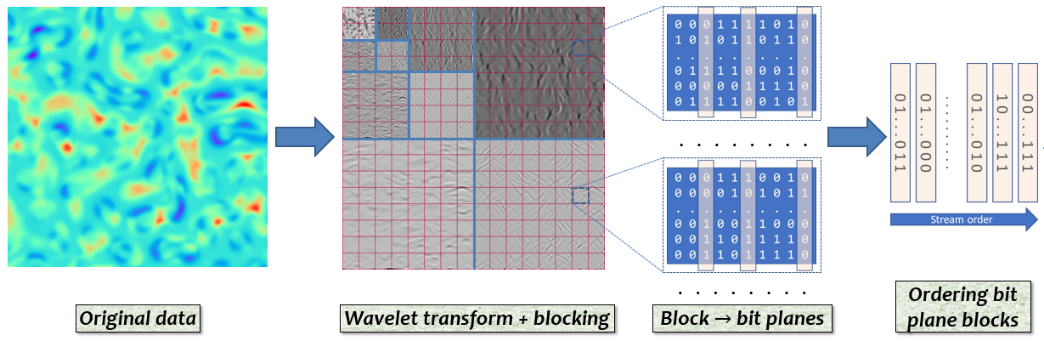
\includegraphics[width=\linewidth]{img/pipeline.png}
  \caption{Our data stream creation pipeline. The input is a regular grid of floating-point values,
  the output is a stream of chunks, where each chunk is a bit plane from a $4\times 4$ group of
  quantized wavelet coefficients, stored in negabinary format. The subbands are separated by blue
  lines in the second image, with the coarsest subband at the top left corner. TODO: revise this
  figure}
  \label{fig:pipeline}
\end{figure}

As mentioned earlier, our unit for streaming is called a \emph{packet} of bits. Precisely, a packet
consists of bits that belong to the same bit plane, from a group of $g^3$ negabinary wavelet
coefficients in the same subband. In this paper, $g=16$, meaning a packet contains $16$ bits. This
choice is based on the fact that, for performance reason, bits are often read and transmitted in
bunch in practice. We have also found that using a packet size of 16 significantly speeds up
experiments without affecting the results in a meaningful way. From its definition, a packet can
always be associated with a subband $l$ ($0\leq l\leq \bar{l}$) and a bit plane $b$ ($0\leq b\leq
\bar{b}$). Different streams can thus be compared based on whether they prioritize packets belonging
to finer subbands (which improves resolution) or packets belonging to lower-ordered bit planes
(which improve precision). The rest of the paper discusses different streams for various analysis
tasks, and compare them on this basis. We use the convention that higher subband is finer (so $l=0$
means the coarsest subband), and higher bit plane is more precise (so $b=0$ is the most significant
bit plane).

\subsection{Data-dependent and data-independent streams}
\label{sec:static-dynamic-streams}

In our data streaming model, there is a ``server'' which serves data and a ``client'' which receives
data from the server. While they can be on the same machine, the server has full knowledge of the
data, but the client does not. Thus, when the client receives a chunk, it might not know where the
chunk should be deposited. A common solution to this problem is to have both the client and the
server agree beforehand on a static ordering of chunks, regardless of the data. We use the term
\emph{static stream} to refer to streams using this solution. In constrast, a \emph{dynamic stream}
is one in which the client is assumed to ``magically'' know the positions of chunks without any
prior agreement with the server. In theory, dynamic streams perform better than static streams
because they can use actual chunk values, not just chunk positions, to better prioritize important
chunks. However, including positions also means that dynamic streams are ill-suited for implementations, because in
practice, the cost associated with sending position information likely outweights any potential
benefit gained from better prioritization of chunks. Despite that, dynamic streams are studied in
this paper because they can serve as a benchmark to evaluate the performance of their static
counterparts.

A stream can be viewed as a collection of chunks, sorted in descending order by weight
associated with each chunk $c$. In the literature, two of the most common orderings are \emph{by
level} and \emph{by bit plane}. The \emph{by level} stream orders the chunks strictly from coarser
to finer resolution levels. The weight function used by this stream is $W_1(c)=\bar{l}-L(c)$, where
$L$ is a function that returns the subband of a given chunk $c$ (with $0$ being the coarsest), and
$\bar{l}$ is the total number of subbands. Within the same subband, without any assumption on the
underlying data, the chunks naturally follow the row-major order. The other common ordering,
\emph{by bit plane}, proceeds strictly from higher-ordered to lower-ordered bit planes. That is,
$W_2(c)=\bar{b}-B(c)$, where $B$ is a function that map a chunk $c$ to the corresponding bit plane
and $\bar{b}$ is the total number of bit planes, with $0$ being the most significant.

The \emph{by level} and \emph{by bit plane} streams are designed to mimic the way data is progressively
accessed in traditional methods that work either in resolution (\emph{by level}) or in
precision (\emph{by bit plane}). We also define a third stream, called \emph{by
wavelet norm}, which combines these two dimensions. The \emph{by wavelet norm} stream orders chunks using
$W_3(c)=2^{\bar{b}-1-B(c)}\times \norm{\omega_{L(c)}}^2$. The term $2^{\bar{b}-1-B(c)}$ captures the
contribution of a bit on bit plane $B(c)$, while the term $\norm{\omega_{L(c)}}^2$ captures the
contribution of a coefficient on subband $L(c)$, where $\omega_{L(c)}$ refers to the wavelet basis
function on subband $L(c)$. The intuition behind \emph{by wavelet norm} is simply that in the
wavelet representation, a function $f$ is written as a linear sum of wavelet basis functions:
$f=\sum{c_i\omega_i}$, where $c_i$ are the coefficients and the basis functions $\omega_i$ in the
same subband have the same norm. Thus $W_3(c)$ is simply the contribution (in $L_2$ norm) of a bit
on bit plane $B(c)$ and subband $L(c)$ to the whole function $f$.

All the three streams mentioned so far are static. In addition, we also consider a
\emph{signature}-based stream to be static. A signature-based stream is one in which the server and
the client establish the agreement over chunk ordering through the transmission of a negligibly
small message, called signature, before any actual value bits are transmitted. A signature is a 2D
array with $\bar{l}$ rows and $\bar{b}$ columns, encoding the relative ordering of all possible
pairs $<l,b>$ for $0\leq l \leq \bar{l}$ and $0\leq b \leq \bar{b}$. We will show that the use of
such signatures can sometimes result in significant improvements over using purely static streams.
Section \ref{sec:stream-signature} gives a detailed discussion of the signature concept.

\subsection{Constructing data-dependent, task-optimized streams}
\label{sec:data_dep_streams}

Each analysis task potentially requires a fundamentally different stream for optimal results. This
section aims to solve the problem of finding the optimal stream, given a data set and
an error metric associated with the analysis task. An error metric is a function
$E(Q(f'),Q(f))$ that returns the distance between its two arguments. $f$ is the original data field
and $f'$ is a reconstructed version of $f$ using a subset of the bits. $Q$ is a quantity of interest
(e.g., histogram, isocontour, etc) derived from $f$ or $f'$. There can be multiple error functions
$E$ for the same $Q$. We choose to use only one error metric with
each quantity, one which is either common, or intuitive and simple while generalizable.
The list of quantity-optimized streams studied in this paper includes \emph{rmse-optimized} (Section
\ref{sec:rmse-optimized}), \emph{gradient-optimized} (Section \ref{sec:gradient}),
\emph{laplacian-optimized} (Section \ref{sec:laplacian}), \emph{histogram-optimized} (Section
\ref{sec:histogram}), and \emph{isocontour-optimized} (Section \ref{sec:isocontour}).

Studying a (data-dependent) quantity-optimized stream is important because such a stream serves both
as a benchmark, and a source of insights for other, more practical streams for the same quantity.
One way to define the ``optimal'' stream for a quantity $Q$ could be the stream that incurs the
minimum error $E$ at every point. However, in trying to realize it, our experience has been that
such a stream does not exist. Assume otherwise that the optimal stream exists, then by definition,
it must be possible to construct this stream using the following greedy algorithm\pavol{the algorithm
may fail to construct optimal stream}: start with a pool
of all chunks (and correspondingly an all-zero $f'$\pavol{zeroed?}, and a presumably very high error $E$), pick
the chunk that when enabled, would minimize $E$, and remove it from the pool. Repeatedly pick and
remove the next chunk that minimizes $E$, until the pool is empty. This algorithm can
encounter a situation in which the next chunk that minimizes the error is on a low-ordered bit plane
of a fine-scale coefficient, which contributes almost nothing to the reconstructed function. The
error is minimized because it is kept approximately constant. In this case, it is actually better to
pick a chunk that increases the error slightly, but otherwise contributes a lot more to the
function. In optimization terms, it is necessary to move in a direction that increases the error to
avoid ending in a local minimum.

The optimal stream for an error metric can also be defined as the stream such that the area bounded
by its plotted error curve and the horizontal axis is the smallest. However, the usefulness of such
a definition is limited in practice, because a stream should be able to be terminated at any point
and still be expected to produce an error as small as possible. Therefore, instead of using this
definition of ``optimality'', we slightly modify the greedy algorithm stated above to avoid the
problem of ending in a local minimum. We start with a pool consisting of all the chunks and an
empty stream, and build this stream back-to-front. In particular, at each step, the chunk whose
removal from the pool has the least impact on the error $E$ is removed and inserted to the beginning
of the current stream. This algorithm solves the problem of unimportant chunks being picked too
early in the original algorithm, because here, chunks picked early are at the end of the
stream, not the beginning.

For our experiments, however, this back-to-front greedy algorithm is too costly. Ignoring
all the steps done in each iteration, this algorithm amounts to a 2-level nested loop running for
$n^2$ iterations, where $n$ is the number of chunks. In 2D, with a $256^2$ data set, a chunk size
that spans $16$ coefficients, and $16$ bits of quantization, $n^2$ would be in the billions, which
we have found to be prohibitively large. We have therefore adopted a simplified version of this
algorithm, where only one pass through the set of $n$ chunks is needed, reducing the number of
iterations from $n^2$ to $n$. The modified algorithm works as follows. We disable (set to zero) a
new chunk $c_i$ in iteration $i$, then compute and record the error $E_i$ due to chunk $c_i$
missing, and enable $c_i$ again at the end of iteration $i$. After repeating the same process for
$n$ iterations, each chunk now has an associated weight, $E_i$. The optimal stream, then, is simply
a sorted list of chunks, in decreasing order of the weights. We observed that this simplified
algorithm brings the running time down from days to minutes, while retaining the same quality of the
output stream. The pseudocode of the algorithm is presented in Algorithm~\ref{alg:greedy}.

\begin{algorithm}[h]
  \caption{Computing a task-optimized stream}
  \begin{algorithmic}[1]
    \Inputs{
			An original function $f$\\
			An unordered set of $n$ chunks $C = \{c_i\}, i\in \{0,\dots,n-1\}$\\
			A quantity of interest $Q$, and a distance function $E$}
		\Initialize{A set of weights $\Gamma = \{\gamma_i\}, i\in \{0,\dots,n-1\}$ }
		\For{each chunk $c_i$}
			\State $c_i \gets 0$
      \State Back-transform $C$ to produce a set of wavelet coefficients $W$
			\State Perform inverse wavelet transform on $W$ to produce $f'$
			\State $\gamma_i \gets E(Q(f'),Q(f))$			
			\State Restore $c_i$
		\EndFor
		\State Sort the $c_i$'s in descending order of $\gamma_i$.
		\Output{The $Q$-optimized stream, which is the sorted $C$}
	\end{algorithmic}
	\label{alg:greedy}
\end{algorithm}
\subsection{Data sets}
\label{sec:data-sets}

Table~\ref{tbl:data-sets} contains all the data sets used for experiment in this paper. Note that
during pre-processing, all fields are converted to double-precision floating-point values before
quantization takes place. For ease of demonstration, as well as performance reason, the majority of
our experiments use 2D data sets. Often, these are slices from 3D volumes.
Section~\ref{sec:3d_results} presents our main results for 3D data sets. \pavol{we switched all to 3D right?}

\begin{table*}[t]
  \caption{Data sets used in experiments}
  \centering
  \begin{tabular}{p{0.15\linewidth}p{0.20\linewidth}p{0.15\linewidth}p{0.10\linewidth}p{0.15\linewidth}}
  \hline
  Name & Source & Slice dimension & Type & Citation\\
  \hline
  boiler & combustion simulation& $140\times 148$ & float64 &\\
  euler & fluid simulation& $256\times 1024$ & float64 &\\
  kingsnake & CT scan & $1024\times 795$ & uint8 &\\
  plasma & magnetic reconnection simulation& $512\times 512$ & float32 &\\
  marschner-lobb & analytical function& $256\times 256$ & float64 &\\
  diffusivity & hydrodynamics simulation& $384\times 384$ & float64 &\\
  pressure & hydrodynamics simulation& $384\times 384$ & float64 &\\
  velocityz & hydrodynamics simulation& $384\times 384$ & float64 &\\
  turbulence & fluid dynamics simulation& $256\times 256$ & float32 &\\
  \hline
  \end{tabular}
\label{tbl:data-sets}
\end{table*}

\subsection{Stream signatures}
\label{sec:stream-signature}

To analyze the core characteristics of a stream, we introduce the concept of a \emph{stream
signature}. A signature is a $\bar{l} \times \bar{b}$ matrix, with $\bar{b}$ being the number of bit
planes, and $\bar{l}$ the number of wavelet subbands. The $(l,b)$ element of the matrix is
associated with chunks belonging in subband $l$ and bit plane $b$ , and contains an integer value in
the range $[0,\bar{b}\times \bar{l})$. This value indicates, on average, the position in which
chunks associated with that element appear in the stream, relative to chunks associated with other
elements. For example, the signature  $A=\bigl[
\begin{smallmatrix}0 & 1 & 4\\ 2 & 3 & 5\end{smallmatrix}\bigr]$ conveys the information that the
most important chunks lie on the first bit plane of the first subband ($A(0,0)=0$), followed by
chunks lying on the second bit plane of the first subband ($A(0,1)=1$), then the first bit plane of
the second subband ($A(1,0)=2$), and so on.

To compute a stream signature, we partition the whole domain into several \emph{regions}, compute
one signature per region, then sum all the per-region signatures. Partitioning is needed since it is
only meaningful to compute the relative ordering of chunks if they come from the same (``small''
enough) region. For example, a chunk at one corner of the domain can be streamed before another
chunk at an opposite corner, but this fact contains no useful information. We want a region to be as
small as possible, and define a region to be the spatial volume/area that is covered by a chunk in
the coarsest subband. So, the total number of regions, $\bar{r}$, is the same as the number of
chunks in the coarsest subband. Note that regions exist in the global domain, as they are not
confined to individual subbands. Ideally, the global signature should retain information from all
the per-region signatures, but due to space constraints, we have chosen to condense all the local
signatures by summing them into one signature. This choice results in signatures that are less
meaningful for data that contains a high degree of spatial variability. We have found, however, that
this choice works well for the various data sets used in this paper. If signatures are deemed useful
enough to be deployed in practice, a more sophisticated ``compression'' of the signature stack might
be necessary for the best results. Algorithm~\ref{alg:signature} lists the steps in detail.

\begin{algorithm}[h]
  \caption{Computing a stream signature}
  \begin{algorithmic}[1]
    \Inputs{
			A stream $C=\{c_i\}, i\in\{0,\dots,n-1\}$\\}
		\Initialize{Per-region signature matrix $A_r\gets 0, r\in\{0,\dots\bar{r}-1\}$\\
		Global signature matrix $A \gets 0$}
		\For{each chunk $c_i$}
			\State Let $r$, $b$, $l$ be the region, bit plane, and subband that $c_i$ belongs
			\State $A_r(l,b) \gets A_r(l,b)+i$
		\EndFor
		\For{each region $r$}
			\State Sort the elements of $A_r$
			\State Assign each element of $A_r$ its index after sorting
			\State $A \gets A+A_r$
		\EndFor
		\State Sort the elements of $A$
		\State Assign each element of $A$ its index after sorting
		\Output{The signature matrix $A$}
	\end{algorithmic}
	\label{alg:signature}
\end{algorithm}

Figure~\ref{fig:signature-static} shows renderings of signatures for the three static streams:
\emph{by bit plane}, \emph{by level}, \emph{by wavelet norm}. Each signature is shown as an image of
size $\bar{b}$ (width) $\times \bar{l}$ (height). The signature's $(0,0)$ element, corresponding to
the coarsest subband and the most significant bit plane, maps to the top-left pixel of the image.
The elements' values are mapped to colors on a linear green scale, in which smaller numbers map to
brighter greens. That is, $(l,b)$ pairs that map to brighter pixels are considered more important
and thus appear earlier in stream.

A signature can be used to construct a ``semi-static'' stream, by iterating through the elements of
the signature in ascending order, and streaming all the chunks associated with each current element.
This stream is similar to purely static streams, in the sense that the ordering of subband-bit plane
pairs is deterministic. However, it is different from purely static streams in that this
deterministic ordering must be established between the client and the server through the
transmission of the signature. Fortunately, the size of the signature is often negligible compared
to the size of the data itself. In 3D, assuming 22 subbands and 32-bit quantized coefficients, a
signature is merely $1408 (=22\times 32\times 2)$ bytes.
